\documentclass[11pt]{article}
\usepackage[margin=1in]{geometry}
\usepackage{amsmath,amssymb,graphicx,booktabs,multirow,array,pdflscape,longtable,tabularx}
\usepackage[numbers]{natbib}
\usepackage{caption}
\usepackage{hyperref}

\title{Online Supplement: Anchoring Large Language Models to Empirical Behavioral Evidence: A Hybrid Approach for Vaccination Uptake Simulation}
\author{Blinded for peer review}
\date{}

\begin{document}
\maketitle

This supplement contains technical appendix material referenced in the main manuscript: derivation details, sensitivity analyses, and replication code listings.

\appendix
\section{Technical Details}
\paragraph{Construction of the Empirical Behavioral Reference (Detailed)}

\medskip

Inference-time regularization requires a deterministic behavioral reference for every policy scenario. For the main experiments, we therefore construct a $4\times4\times4=64$-state evaluation grid by varying waiting time, vaccine efficacy, and side-effect risk across four levels each while fixing the cash incentive and vaccine origin at their reference levels. The behavioral reference is computed using the MLE coefficients of the corrected 6-parameter grouped/conditional logit (five attribute coefficients plus an opt-out alternative-specific constant) on the full DCE sample; the canonical utility specification used throughout this paper is reported in Section~3.2 of the main manuscript and includes all five DCE attributes (waiting time, vaccine efficacy, side-effect risk, cash incentive, vaccine origin) plus the opt-out ASC:

\[
U(x, \bar\beta) = \bar\beta_{\mathrm{wait}}\mathrm{WaitTime} + \bar\beta_{\mathrm{eff}}\mathrm{Efficacy} + \bar\beta_{\mathrm{side}}\mathrm{SideEffects} + \bar\beta_{\mathrm{cash}}\mathrm{Cash} + \bar\beta_{\mathrm{origin}}\mathrm{Origin},
\]
where $\bar\beta$ is the MLE coefficient vector and $\hat\beta_{\mathrm{ASC}}$ is the MLE estimate of the opt-out alternative-specific constant (coded 1 for opt-out and 0 for all non-opt-out alternatives during estimation). The 64-state grid varies waiting time, vaccine efficacy, and side-effect risk across four levels each while holding cash incentives at 0 RMB and vaccine origin at its reference level, so on the 64-state grid these two terms equal zero under the reference coding (cash = 0, origin = 0); the opt-out utility is represented separately by the ASC $V_{\mathrm{opt-out}} = \hat\beta_{\mathrm{ASC}}$, identified through the opt-out contrast and surfacing as a separate additive constant in the choice-probability ratio rather than as an attribute absorbed into the policy utilities.

\[
P_{\mathrm{emp}}(y=1\mid\mathbf{x})
=
\sigma\!\bigl[U(\mathbf{x}, \bar\beta) - \hat\beta_{\mathrm{ASC}}\bigr].
\]

This deterministic utility-based approximation preserves the ordinal structure and directional monotonicity of the empirical choice frontier while providing a stable and computationally efficient behavioral reference for inference-time regularization.
\subsection{Stage 2: Inference-Time Adjustment Procedure (Detailed)}

\label{sec:stage2}

Given the empirical behavioral reference from Stage~1, the second stage adjusts LLM-generated choice probabilities after generation. Rather than retraining the LLM, the proposed approach operates entirely after generation, combining the LLM's prediction with empirically estimated behavioral knowledge.

For each policy scenario $\mathbf{x}_g$, the LLM is prompted to evaluate the vaccination decision from the perspective of a decision-maker and report a choice probability. Let $\pi_{\mathrm{LLM}}(y=1\mid\mathbf{x}_g)$ denote the LLM-generated probability. To reduce variation, probabilities are averaged over multiple generations.

The adjusted probability is then defined as

\begin{equation}
\pi_{\mathrm{adj}}(y=1\mid\mathbf{x}_g) = \lambda \cdot \pi_{\mathrm{LLM}}(y=1\mid\mathbf{x}_g) + (1-\lambda) \cdot P_{\mathrm{emp}}(y=1\mid\mathbf{x}_g),
\label{eq:adjustment}
\end{equation}

where $\lambda \in [0,1]$ controls the relative weight given to the LLM versus the empirical reference, and $P_{\mathrm{emp}}(y=1\mid\mathbf{x}_g) = \sigma(U(\mathbf{x}_g) - \beta_{\mathrm{ASC}})$ is the DCE-implied binary policy-versus-opt-out probability under the conditional logit model (i.e., the probability of choosing the policy alternative over the opt-out, given the policy attributes $\mathbf{x}_g$). This quantity is a model-implied empirical reference score that depends on the IIA assumption for choice-set extrapolation from the original three-alternative DCE design; it is not a directly observed absolute acceptance probability from the original experiment. The held-out DCE log loss and Brier score are reported as sensitivity diagnostics and were not used to select $\lambda$; the value is not a test-set-optimized predictive optimum.

The adjustment has intuitive limiting cases: $\lambda=1$ corresponds to the unconstrained LLM, while $\lambda=0$ reduces to the pure DCE model.

Because the adjustment operates after generation, it requires no modification of the underlying LLM. All components---the raw LLM probability, empirical reference, weight, and adjusted probability---are explicitly observable, making the procedure transparent and auditable. It can be applied to any LLM without retraining.

\renewcommand{\thetable}{S\arabic{table}}
\setcounter{table}{0}

\section{Pure-Noise LLM Null Distribution}
\label{sec:null_distribution}

To interpret the frontier-alignment Spearman $\rho(\pi_{\text{EFR}}, P_{\text{emp}})$ reported in Table~1 of the main text and Table~\ref{tab:lambda_frontier} of this supplement, we generated a Monte Carlo null distribution by replacing the LLM component with a uniform random draw $U[0, 1]$ on each of 10{,}000 replicates, then computing $\rho(0.25 \cdot U + 0.75 \cdot P_{\text{emp}},\ P_{\text{emp}})$ against the empirical $P_{\text{emp}}$ surface. The resulting null distribution has mean $\rho = 0.367$ (SD = 0.099; 95% CI $[0.147,\,0.566]$) for the structured extrapolation 64-state grid and mean $\rho = 0.89$ (SD = 0.06) for the tied Panel B (OOD) surface, in which only six distinct empirical $P_{\text{emp}}$ values appear across 28 scenarios, mechanically pushing rank correlations toward the high end of the unit interval regardless of the LLM component. The reported frontier-alignment value on the 64-state grid ($\rho = 0.6886$ for Qwen2.5-72B-Instruct; $\rho = 0.7558$ for MiroThinker-1.7-mini; point estimates from Table~\ref{tab:lambda_frontier} of this supplement, mirroring Table~1 of the main text) exceeded the null mean for both models, with the rank-correlation panel reported in Table~1 of the main text and in Table~\ref{tab:lambda_frontier} best read as a structural diagnostic of how closely the EFR blend tracks the empirical frontier, not as a behavioral significance test. The reported OOD frontier-alignment values ($\rho = 0.87$--$0.93$ for Qwen; $\rho = 0.87$--$0.88$ for DeepSeek V4) sit inside one SD of the tied null and should be read as descriptive structural robustness measures rather than as a behavioral finding. The fairer benchmark---held-out DCE log loss---is reported in Section~4.2 of the main text.

\section{ELEVATE-GenAI Reporting Details}
\label{app:elevate_genai}

This appendix documents compliance with the ViH/ISPOR ELEVATE-GenAI reporting framework for generative-AI evaluations in health-economics and outcomes research. The framework requires itemized reporting of model identity, endpoint, access date, decoding parameters, prompt template, output parser, and missing-output handling for every LLM evaluation reported in the manuscript.

\paragraph{Model identity, endpoint, and access dates.}
\begin{table}[h]
\centering
\caption{LLM decoding and endpoint parameters used in the main, supplementary, and stress-test evaluations.}
\label{tab:llm_decoding}
\footnotesize
\setlength{\tabcolsep}{3pt}
\renewcommand{\arraystretch}{1.15}
\begin{tabularx}{\textwidth}{@{}>{\raggedright\arraybackslash}p{2.25cm} >{\raggedright\arraybackslash}p{2.15cm} >{\centering\arraybackslash}p{1.55cm} >{\centering\arraybackslash}p{1.05cm} >{\centering\arraybackslash}p{0.85cm} >{\centering\arraybackslash}p{1.05cm} >{\centering\arraybackslash}p{0.45cm} >{\raggedright\arraybackslash}X@{}}
\toprule
\textbf{Model} & \textbf{Endpoint / Provider} & \textbf{Access date} & \textbf{Temp.} & \textbf{top-$p$} & \textbf{\shortstack{Max\\tokens}} & \textbf{$R$} & \textbf{Notes} \\
\midrule
Qwen2.5-72B-Instruct       & Hugging Face Inference API            & 2026-05-19            & 0.7    & 1.0 & 512    & 10 & Full-scale primary; Main Table 1; Tables S5--S6 \\
DeepSeek V4                & Provider inference API                & 2026-05-19            & 0.7    & 1.0 & 512    & 10 & Full-scale robustness; Main Table 1; Table S5 \\
MiroThinker-1.7-mini       & Provider inference API                & 2026-05-19            & 0.0    & 1.0 & 256    & 10 & Full-scale robustness (deterministic); Main Table 1; Table S5 \\
\midrule
Qwen2.5-1.5B               & Ollama (local; Mac mini, 8\,GB)       & 2026-04              & 0.7    & 1.0 & 256    & 5  & NDS pilot only (the main text); n=2 prompts \\
\midrule
Qwen2.5-72B-Instruct       & Ollama (local; Mac Studio, qwen2.5:72b) & 2026-09-10           & 0.7    & 1.0 & 512    & 10 & Exact-task multinomial validation; quantized implementation differs from HF API \\
\midrule
Qwen2.5-7B                 & Local vLLM                            & 2026-08-13           & 0.7    & 1.0 & 512    & 10 & Stress test (8 Panel~B scenarios); degenerate output documented in Section~4.3 \\
DeepSeek V4 (Flash variant)& Provider inference API                & 2026-08-13           & 0.7    & 1.0 & 512    & 10 & Stress test (8 Panel~B scenarios); 0\% parse on N1 documented in Section~4.3 \\
\bottomrule
\end{tabularx}
\end{table}

The 640 generations per model the full-scale run logs report are the product of 64 policy states $\times$ $R=10$ repeated generations per state for each of the three full-scale models; the 1{,}920 total full-scale generations are pooled across the three models. The $R=10$ repetition is required to average out sampling noise under non-zero decoding temperature; identical prompts and decoding settings (other than the temperature/top-$p$/max-tokens entries above) are reused across the three models to make the cross-model comparison strictly fair. The system prompt template is:

\begin{quote}\small\ttfamily
You are evaluating a vaccination decision. The respondent is deciding whether to accept the proposed COVID-19 vaccine. Read the policy description below and decide.

Decision: Yes or No

Probability: a number between 0 and 100

Reasoning: one sentence.
\end{quote}

Failed parses were excluded from the current state mean. Failed state--replicate combinations could be regenerated during checkpoint/resume runs; no probability-value imputation was performed. In practice this case did not arise in the full-scale data: each of the 64 states has at least one parseable replicate for all three models.

\paragraph{Robustness, reproducibility, and deployment context.}
The empirical frontier coefficients reported in Table~S4 are computed once on the full Wuhan DCE sample ($N = 1{,}027$; $N_{\text{choice}} = 6{,}162$) for the main 64-state grid evaluation; they are not re-estimated inside the LLM simulation loop. \textbf{For the held-out validation (Table~S16), all DCE components---including the empirical frontier used in EFR ($P_{\text{emp,train}}$)---are estimated exclusively from the 822 training respondents.} Calibration of the Static-BDT anchor at $\lambda=0.25$ is reported in Tables~S4 and S5. The validation hierarchy is: \textbf{(i) primary predictive validation:} exact-task 3-alternative multinomial log loss on six canonical DCE tasks ($N = 205$ respondents, 1,230 choices); \textbf{(ii) secondary sensitivity:} 813-row alternative-level binary log loss/Brier/AUC (Supplementary Material Table~S6); \textbf{(iii) structural diagnostics:} frontier-alignment Spearman $\rho$ and waiting-time MVR. The model's intended use is a behavioral-consistency layer for LLM-based policy simulators, not as a substitute for primary stated-preference data collection; deployment context (single Wuhan DCE, single jurisdiction, single-decision choice task) is documented in the main Limitations paragraph.

\paragraph{Accuracy, regularization, and external validation.}
Accuracy is reported in three complementary ways: (i)~within-design \emph{alternative-level} log loss and Brier on the LLM-matched held-out subset ($N=813$ alternative-level binary-outcome rows from $N=205$ held-out respondents; each row is one of three alternatives within one of six tasks, with $y \in \{0,1\}$ indicating whether the respondent selected that alternative). The full held-out pool contains $N=3{,}690$ alt-rows (1{,}027 respondents $\times$ 6 tasks $\times$ 3 alternatives); after excluding one anomalous wait=2 alt-row from a single respondent, 3{,}689 rows remain under the intended design; of these, 813 are matched and 2{,}876 are unmatched. The 813-row matched subset is the literal overlap between the intended DCE design and the LLM grid on the three focal attributes (waiting time, efficacy, and side-effect burden), populating 11 of 12 candidate cells; (ii)~Spearman rank correlation with the empirical frontier on the 64-state grid and on the 8-pair OOD-narrative surface; and (iii)~a structural diagnostic of the 75\% $P_{\text{emp}}$ blend: the share of 15 unordered policy pairs with matching rank order to Pure-DCE (no confidence interval, no significance test, because the 15 pairs share six underlying policy effects). Probabilistic predictive performance is reported in the convex-blend $\lambda$ sensitivity in Table~S5; the Static-BDT anchor trades a 0.020 within-design log-loss gap against improved rank alignment and improved OOD-narrative robustness. External validation is limited to a single Wuhan DCE; replication across additional jurisdictions and decision contexts is documented as a future-work item. The full code and supporting files, including prompt templates, parsed outputs, raw LLM traces, and analysis scripts, are publicly available at \url{https://github.com/REDACTED/behavioral-digital-twins}.

\section{DCE Attribute Levels and Static Frontier Estimates}
\label{app:dce_attributes}

\paragraph{DCE design per ISPOR Good Practices checklist~\citep{Johnson2013DCE, Hauber2016DCE, Marshall2016DCE, Bridges2013DCE}.} \emph{The administered DCE attribute levels and the attribute coding dictionary are reported in Tables S2 and S3 below; the design is summarized in the Methods section of the main text and reproduced for self-containment here.} The Wuhan vaccination-timing DCE used a \textbf{non-orthogonal fractional design}. The intended non-opt-out candidate space contained 216 profiles (4 wait $\times$ 3 efficacy $\times$ 3 side-effect $\times$ 3 cash $\times$ 2 origin levels, namely waiting time $\in \{0, 1, 3, 6\}$, vaccine efficacy $\in \{0.5, 0.7, 0.95\}$, side effects (risk) $\in \{0.1, 1, 10\}\%$ coded as $\{1, 2, 3\}$, cash incentive $\in \{50, 200, 800\}$, and vaccine origin $\in \{\text{Domestic}, \text{Imported}\}$). \emph{All 1,027 respondents completed the same six choice tasks, each presenting two non-opt-out alternatives and an opt-out alternative. The design therefore contained six unique administered choice tasks and 12 non-opt-out profiles.} The 12 administered non-opt-out attribute combinations per respondent enumerate 12 of the 216 non-opt-out candidate cells (5.6\% coverage). \emph{The raw coded data ($N=18{,}486$ alt-rows) contain one additional 1-row outlier at wait $= 2$ months from a single respondent; this row is excluded from the non-opt-out candidate space because wait $= 2$ months is not an administered design level and the row is inconsistent with the design matrix.} The full per-attribute level distribution is reported in the methods narrative of the main text and in Table~\ref{tab:dce_attributes} below. Willingness-to-pay (WTP) is \emph{not} reported in this paper. The WTP calculation depends on the unit of the cash-incentive coefficient, which is sensitive to the choice of payment-level scaling (50/200/800 vs 0/50/200/800, linear vs log specification); a robust WTP estimate is out of scope for the present methodological contribution and will be reported in a separate applied-economics note. The conditional-logit coefficient ratio is, however, reported in Table~\ref{tab:static_frontier_estimates}. The 64-state evaluation grid retains only the three focal attributes at four levels each, with cash incentive fixed at 0 RMB and vaccine origin fixed at ``reference'' framing; the empirical frontier is estimated jointly over the five attributes in the DCE, so the frontier coefficients reflect the full 216-profile non-opt-out candidate space.

This appendix documents the attribute structure of the Wuhan vaccination-timing discrete choice experiment (DCE) and the static conditional-logit estimates used to construct the empirical choice frontier in the main analysis. The full DCE instrument varied five policy-relevant attributes: waiting time, vaccine efficacy, side-effect risk, cash incentives, and vaccine origin. The main 64-state evaluation grid used in the full-scale BDT experiments focuses on three focal attributes (waiting time, vaccine efficacy, side-effect burden) and holds cash incentives and vaccine origin at their reference values; the corrected 6-parameter specification additionally includes an alternative-specific constant for the opt-out alternative. These attributes define the policy grid on which the unconstrained LLM and Static-BDT Anchor are evaluated in Table~1 of the main text.

\subsection{DCE Attribute Levels}

Table~\ref{tab:dce_attributes} reports the attribute levels used in the DCE. Waiting time and side-effect burden are disutility attributes: higher values are expected to lower vaccine acceptance. Vaccine efficacy and cash incentives are utility-enhancing attributes: higher values are expected to increase vaccine acceptance.

\begin{table}[htbp]
\centering
\caption{DCE attribute levels.}
\label{tab:dce_attributes}
\begin{tabular}{lll}
\hline
Attribute & Levels (administered / non-opt-out) & Expected direction \\
\hline
Wait Time (months) & 0, 1, 3, 6 (non-opt-out design levels; the raw coded data contain a single 1-row outlier at wait $= 2$ months which is excluded from the non-opt-out candidate space because it does not represent an administered design level) & Negative \\
Vaccine Efficacy & 0\%, 50\%, 70\%, 95\% (non-opt-out: 50\%, 70\%, 95\%) & Positive \\
Side Effects (\% risk) & 0.1, 1, 10 (non-opt-out only; 0\% not administered) & Negative \\
Cash Incentive (RMB) & 50, 200, 800 (administered); 0 only as opt-out & Positive \\
Vaccine Origin & Imported, Domestic & (binary) \\
\hline
\end{tabular}
\end{table}

\subsection{Static Empirical Choice Frontier}

The empirical frontier used in the main full-scale experiment is constructed using a \textbf{6-parameter grouped/conditional logit with five attribute coefficients and an opt-out alternative-specific constant} on the full DCE sample. The corrected specification trades random-coefficients heterogeneity for a behaviorally honest treatment of the opt-out alternative, and is the canonical frontier reported throughout the main text.

For the construction of the 64-state evaluation grid and the computation of the Static-BDT anchor, the systematic utility for alternative $x$ is strictly specified as the five-attribute linear index (without the opt-out indicator; the opt-out contrast is identified through the ASC coefficient and surfaces as a separate additive constant in the choice-probability ratio):
\[
U(x, \bar\beta) = \bar{\beta}_{\mathrm{wait}}\mathrm{WaitTime} + \bar{\beta}_{\mathrm{eff}}\mathrm{Efficacy} + \bar{\beta}_{\mathrm{side}}\mathrm{SideEffects} + \bar{\beta}_{\mathrm{cash}}\mathrm{Cash} + \bar{\beta}_{\mathrm{origin}}\mathrm{Origin},
\]
where the ASC is identified in the estimation by coding the opt-out alternative as 1 and all non-opt-out alternatives as 0, but enters the choice-probability expression as a separate additive constant (not as an attribute of $U$). All five attributes enter linearly; no random parameters are specified in the corrected 6-parameter specification. Under conditional logit with the opt-out alternative treated as the reference category, the choice probability of accepting policy $x$ against the opt-out alternative is the sigmoid of the utility gap:
\[
P_{\mathrm{emp}}(y=1|x) = \frac{\exp\!\bigl[U(x, \bar\beta)\bigr]}{\exp\!\bigl[\hat\beta_{\mathrm{ASC}}\bigr] + \exp\!\bigl[U(x, \bar\beta)\bigr]} = \sigma\!\bigl[U(x, \bar\beta) - \hat\beta_{\mathrm{ASC}}\bigr],
\]
where $\bar\beta$ is the MLE coefficient vector. The 64-state grid is constructed by varying waiting time, vaccine efficacy, and side-effect risk across four levels each while fixing cash incentives and vaccine origin at their reference levels. Including the opt-out ASC, the corrected 6-parameter specification yields a $P_{\mathrm{emp}}$ range of $[0.47, 0.64]$ across the 64-state grid. (A 5-parameter conditional logit fitted without the opt-out ASC would produce a wider $P_{\mathrm{emp}}$ range of $[0.27, 0.71]$, but is not the canonical specification used in this paper.)

\subsection{Coding Dictionary and Unit Reconciliation}
\label{sec:coding_dict}

Table~\ref{tab:coding_dict} reports the full attribute coding used in this paper. Five columns are reported side-by-side to remove any ambiguity about the unit at each stage of the analysis pipeline: (i)~the DCE questionnaire display value the respondent sees; (ii)~the value that is actually passed as the independent variable into the conditional-logit likelihood; (iii)~the DCE coefficient unit (i.e., the per-unit change in utility per one-unit change in the value in column~(ii)); (iv)~the value passed to the utility function on the 64-state evaluation grid; and (v)~the grid display value that the unconstrained LLM is asked to evaluate. \emph{Three scale decisions matter and are reported explicitly because they are easy to misread:}

\begin{enumerate}
\item \textbf{Vaccine efficacy} is reported in the DCE questionnaire as $\{0, 50, 70, 95\}\%$ and in the 64-state grid as $\{30, 50, 70, 90\}\%$; the two supports share the literal overlap $\{50\%, 70\%\}$ used for held-out matching. The estimated coefficient $\hat\beta_{\text{eff}}$ is reported in Table~\ref{tab:static_frontier_estimates}; the coefficient unit is the same coded value that enters the linear predictor (proportion, so $\hat\beta_{\text{eff}} = 0.4153$ is per 1.0 proportion, i.e., per 100 percentage points).

\item \textbf{Side-effect burden} is reported in the DCE questionnaire as $\{0.1, 1, 10\}\%$ risk of the listed side effect, coded as $\{1, 2, 3\}$ in the analytic data (level 0 was not administered). The estimated coefficient $\hat\beta_{\text{SE}}$ is reported in Table~\ref{tab:static_frontier_estimates}; the coefficient unit is the coded burden level that enters the linear predictor.
\item \textbf{Waiting time} is coded in months throughout (DCE: $\{0, 1, 3, 6\}$ -- the four real design levels; grid: $\{0, 2, 4, 6\}$); $\hat\beta_{\text{wait}} = -0.0590$ is per 1 month in both. \emph{The raw coded DCE data contain a single 1-row outlier at wait $= 2$ months from one respondent which is excluded as a data anomaly.}
\end{enumerate}

The cash-incentive attribute is held at $0$ RMB in the 64-state grid (the LLM and Static-BDT comparison absorbs the cash coefficient into the opt-out alternative-specific constant); the vaccine-origin attribute is held at the reference (domestic) framing. The full DCE estimation column-(ii) values are reported for completeness.

\begin{table}[h]
\centering
\caption{Attribute coding dictionary: DCE questionnaire display, value passed into the conditional-logit likelihood (column~(ii)), the 64-state grid value passed into the utility function (column~(iv)), and the DCE coefficient unit. \emph{The SE column-(iv) grid value uses the same integer-coded burden scale as the estimation variable; the LLM prompt presents the column-(iv) value to the model.}}
\label{tab:coding_dict}
\scriptsize
\setlength{\tabcolsep}{3pt}
\renewcommand{\arraystretch}{1.20}
\begin{tabularx}{\textwidth}{>{\raggedright\arraybackslash}p{0.11\textwidth} >{\raggedright\arraybackslash}p{0.17\textwidth} >{\raggedright\arraybackslash}p{0.16\textwidth} >{\raggedright\arraybackslash}p{0.13\textwidth} >{\raggedright\arraybackslash}p{0.20\textwidth} >{\raggedright\arraybackslash}p{0.13\textwidth}}
\toprule
\textbf{Attribute} & \textbf{DCE display (respondent)} & \textbf{Value passed to clogit (column ii)} & \textbf{DCE coef unit} & \textbf{Grid value passed to utility (column iv)} & \textbf{LLM prompt display} \\
\midrule
Waiting time & 0, 1, 3, 6 months & 0, 1, 3, 6 (raw months; the raw coded data contain one additional 1-row outlier at wait $= 2$ months which is excluded) & per 1 month & 0, 2, 4, 6 (raw months) & 0, 2, 4, 6 months \\
\midrule
Vaccine efficacy & 0\%, 50\%, 70\%, 95\% & 0.0, 0.5, 0.7, 0.95 (proportion) & per 1.0 proportion (i.e., per 100 percentage points in questionnaire display) & 0.3, 0.5, 0.7, 0.9 (proportion) & 0.3, 0.5, 0.7, 0.9 \\
\midrule
Side-effect burden & 0.1\%, 1\%, 10\% & 1, 2, 3 (integer-coded burden level; level 0 not administered) & per 1 coded burden level & 1, 2, 3 (integer-coded burden level) & 0.1\%, 1\%, 10\% \\
\midrule
Cash incentive & 0, 50, 200, 800 RMB & 0, 50, 200, 800 (raw RMB) & per 1 RMB & 0 RMB (held; contribution to $U$ = 0) & 0 RMB (held) \\
\midrule
Vaccine origin & Domestic, Imported & 0 (Domestic) / 1 (Imported) & per 1 step (Imported) & 0 (reference; held) & 0 (reference) \\
\midrule
Opt-out & N/A & Alternative-specific constant (1 for opt-out) & per 1 opt-out step & ASC (held) & -- \\
\bottomrule
\end{tabularx}
\end{table}

\subsection{Conditional-Logit Estimates}

\textbf{Preprocessing rule.} One anomalous alternative-level row (RespondentID~1, task~1, wait~$=2$ months, a level not administered in the DCE design matrix) is excluded from the raw coded data before \emph{all} estimation, before the 64-state frontier fit, and before the held-out respondent split; no analysis reported in this paper uses the wait$=2$ row. The single explicit exclusion is applied uniformly across the full-sample frontier coefficients (Table~\ref{tab:static_frontier_estimates}), the data-scaling ablation (Table~\ref{tab:data_scaling_benchmarks}), and the held-out DCE predictive validation (Table~\ref{tab:lambda_heldout}).

Table~\ref{tab:static_frontier_estimates} reports the static conditional-logit estimates used to construct the empirical choice frontier. The signs follow the expected behavioral directions: waiting time and side effects reduce acceptance, while vaccine efficacy and cash incentives increase acceptance.

\begin{table}[h]
\centering
\caption{Conditional-logit estimates (corrected 6-parameter specification) used to construct the empirical choice frontier. Coefficients are displayed to four decimals; the frontier probabilities and all downstream metrics are computed from the underlying six-decimal estimates, so re-computing $P_{\text{emp}}$ from the rounded values below reproduces the frontier only to display precision. \emph{Estimates are from a single fit on the full DCE sample after excluding one anomalous wait=2 alt-row before all estimation ($N = 1{,}027$ respondents, 6,162 choice tasks (1,027 respondents $\times$ 6 tasks) and 18,485 alternative-level rows (6,162 $\times$ 3 alternatives minus one wait=2 row)) using the canonical 5 attribute variables plus an opt-out alternative-specific constant (Coding A: $\mathrm{ASC} = 1$ for the opt-out alternative and $0$ otherwise).}}
\label{tab:static_frontier_estimates}
\small
\setlength{\tabcolsep}{8pt}
\begin{tabular}{l c c}
\toprule
\textbf{Attribute / Term} & \textbf{Coefficient} & \textbf{S.E.} \\
\midrule
Vaccine Origin & $0.2455^{***}$ & $(0.048)$ \\
Wait Time (months) & $-0.0590^{***}$ & $(0.013)$ \\
Vaccine Efficacy (proportion) & $0.4153^{***}$ & $(0.064)$ \\
Side Effects (coded burden level) & $-0.0357$ & $(0.025)$ \\
Cash Incentive (CNY) & $0.0010^{***}$ & $(0.0001)$ \\
ASC (opt-out) & $-0.2100^{***}$ & $(0.054)$ \\
\bottomrule
\end{tabular}

\vspace{0.4em}
\begin{minipage}{0.95\textwidth}
\small
\textit{Note.} Estimates are from the corrected 6-parameter conditional logit on the full DCE sample ($N=1{,}027$ respondents; effective $N_{\text{choice}} = 6{,}162$ choice observations (1,027 respondents $\times$ 6 tasks, with each task contributing 3 alternatives)). The raw file contains 18,486 alternative-level rows; the analytic sample contains 18,485 after excluding the single anomalous wait=2 row. All five attribute coefficients enter linearly (no random parameters); the opt-out alternative carries an alternative-specific constant (ASC = 1 for opt-out, 0 for non-opt-out alternatives). The cash-incentive and vaccine-origin attributes are held at their reference values in the 64-state grid evaluation, but are estimated jointly with the three focal attributes in the frontier fit. The respondent-cluster bootstrap (2{,}000 replicates, Appendix~\ref{app:bootstrap}) confirms that all six coefficients retain their canonical sign in $\geq 97.7\%$ of replicates; the side effects coefficient has the smallest empirical signal (canonical $\hat\beta_{\text{SE}} = -0.0357$, 95\% CI $[-0.085, 0.014]$). $^{***}p < 0.001$, $^{*}p < 0.05$.
\end{minipage}
\end{table}

All coefficients display the expected sign. The negative coefficient on Wait Time implies that longer waiting time lowers the empirical probability of vaccine acceptance, while the negative coefficient on SideEffects implies that greater side-effect burden lowers acceptance. The positive coefficient on Vaccine Efficacy implies that more effective vaccines are preferred, and the positive coefficient on Cash Incentives implies that larger incentives increase vaccine acceptance. The negative ASC coefficient ($\hat\beta_{\mathrm{ASC}} = -0.2100$, with the ASC coded as $+1$ for the opt-out alternative and $0$ for the non-opt-out alternatives during estimation) means that, holding the policy attributes fixed, respondents are \emph{more} likely to choose the policy than to opt out, not less: under $P_{\mathrm{emp}} = \sigma[U(x, \bar\beta) - \hat\beta_{\mathrm{ASC}}]$, the negative ASC enters the sigmoid as a positive additive constant to the utility gap, so $P_{\mathrm{emp}} > \sigma[U(x, \bar\beta)]$ for any non-opt-out policy $x$, and the probability mass on the opt-out shrinks. Equivalently, $\exp(\hat\beta_{\mathrm{ASC}}) = 0.61 < 1$ indicates that the odds of selecting the opt-out are 0.61 times the odds of selecting a zero-attribute policy profile, conditional on the policy attributes. The corrected 6-parameter specification thus identifies an opt-out aversion among Wuhan respondents, consistent with the high policy-attribute variance in the raw DCE data. These directional restrictions define the monotonicity conditions used to compute MVR-Wait and MVR-SE in the main evaluation.

\subsection{Connection to the 64-State Evaluation Grid}

The 64-state grid used in the full-scale BDT experiments is not a respondent-level train--test split. Instead, it is a fixed full-factorial policy grid over the three focal attributes:

\[
G
=
\{(\text{wait}, \text{eff}, \text{se}) :
\text{wait} \in \{0,2,4,6\},
\text{eff} \in \{0.30,0.50,0.70,0.90\},
\text{se} \in \{0,1,2,3\}
\}.
\]

For each state \(x_g \in G\), the empirical benchmark is

\[
P_{\text{static},g}
=
P_{\text{static}}(y=1 \mid x_g).
\]

The full-scale LLM and Static-BDT results in Table~1 of the main text are evaluated by comparing agent-implied probabilities against \(P_{\text{static},g}\) over this common 64-state grid. This design ensures that all model comparisons are made on the same policy-relevant attribute space.



\section{Pilot Experiment Details}
\label{app:pilot}

This appendix documents the pilot experiment, which served as a low-resource mechanism check rather than a directly comparable full-scale evaluation. It tested whether explicit monotonicity information could reduce frontier-relative behavioral inconsistencies in a minimal setting before scaling to the full Static-BDT Anchor implementation.

\subsection{Pilot Design}

The pilot used a randomly sampled 10\% subset of the DCE respondent data with a fixed random seed. The base model was Qwen2.5-1.5B, deployed locally via Ollama on a consumer-grade Mac mini with 8\,GB of unified memory. The pilot evaluated two conditions:

\begin{enumerate}
    \item \textbf{Unconstrained LLM}: the model was prompted as a patient considering a vaccine, without any explicit behavioral rule.
    \item \textbf{Rule-injection BDT}: the model was prompted with a simple monotonicity rule derived from the DCE logic: longer waiting time should reduce willingness to accept vaccination.
\end{enumerate}

Unlike the full-scale Static-BDT Anchor used in the main experiment, the pilot did not apply the post-generation convex anchoring rule in Eq.~\eqref{eq:adjustment}. Instead, it used prompt-level rule injection. The pilot results should therefore be interpreted as low-resource mechanism evidence that explicit monotonicity information can reduce frontier-relative behavioral inconsistencies, not as a direct estimate of the full frontier-anchored regularization mechanism.

\subsection{Pilot Prompt Templates}

For reproducibility, we document the prompt templates used in the pilot experiment. The pilot varied waiting time while holding the other displayed attributes fixed. This simplified design isolates whether the model respects the expected directional effect of waiting time.

\subsubsection{Unconstrained LLM Baseline}

The unconstrained baseline prompt presented the model as a patient considering vaccination, without any monotonicity rule:

\begin{quote}
\small
You are a patient considering a vaccine.

Waiting time: \{wait\} months.

Cost: \$50.

Risk of mild side effects: 5\%.

Would you accept the vaccine?

You must reply exactly in this format:

Decision: Yes or No

Probability: a number between 0 and 100

Reasoning: one short sentence
\end{quote}

\subsubsection{Rule-Injection BDT Prompt}

The rule-injection BDT prompt added an explicit monotonicity rule before the same decision scenario:

\begin{quote}
\small
You are a behavioral agent in a vaccine policy simulation.

You must follow this behavioral rule derived from discrete choice experiment evidence:

- Longer waiting time decreases willingness to accept.

Scenario:

Waiting time: \{wait\} months.

Cost: \$50.

Risk of mild side effects: 5\%.

Would you accept the vaccine?

You must reply exactly in this format:

Decision: Yes or No

Probability: a number between 0 and 100

Reasoning: one short sentence
\end{quote}

\subsection{Pilot MVR Calculation}

The pilot monotonicity violation rate (MVR) was computed on the waiting-time dimension only. For each pair of pilot states \(x^{(a)}\) and \(x^{(b)}\) that differed only in waiting time, with

\[
\text{WaitTime}^{(a)} < \text{WaitTime}^{(b)},
\]

a violation was recorded if the model assigned a lower choice probability to the shorter-wait alternative than to the longer-wait alternative:

\[
\bar{\pi}(y=1 \mid x^{(a)})
<
\bar{\pi}(y=1 \mid x^{(b)}).
\]

The pilot MVR is therefore

\[
\text{MVR}
=
\frac{
\# \{(x^{(a)},x^{(b)}): \text{WaitTime}^{(a)} < \text{WaitTime}^{(b)}
\ \text{and}\
\bar{\pi}(y=1 \mid x^{(a)}) < \bar{\pi}(y=1 \mid x^{(b)})\}
}{
\# \{(x^{(a)},x^{(b)}): \text{WaitTime}^{(a)} < \text{WaitTime}^{(b)}\}
}.
\]

Each pilot state was queried repeatedly, and the mean predicted probability across repetitions was used when evaluating monotonicity violations. The unconstrained pilot condition produced an MVR of 50.0\%, while the rule-prompted condition reduced MVR to 22.2\%. Because the pilot constrained only waiting time and held other displayed attributes fixed, MVR-SE, MAE, and Spearman \(\rho\) were not computed for the pilot condition.

\subsection{Relationship to the Full-Scale Static-BDT Anchor}

The pilot differs from the full-scale experiment in three important ways. First, the pilot used a smaller 1.5B local model, whereas the full-scale experiment uses Qwen2.5-72B-Instruct as the primary model and includes DeepSeek V4 and MiroThinker-1.7-mini as robustness models. Second, the pilot varied only waiting time while holding cost and side-effect risk fixed, whereas the full-scale experiment evaluates a 64-state grid over waiting time, vaccine efficacy, and side-effect burden. Third, the pilot used prompt-level rule injection, whereas the full-scale Static-BDT Anchor applies a post-generation convex anchoring rule:

\[
\pi_{\text{BDT}}(y=1 \mid x)
=
\lambda \bar{\pi}_{\text{LLM}}(y=1 \mid x)
+
(1-\lambda)P_{\text{static}}(y=1 \mid x).
\]

The pilot therefore provides low-resource mechanism evidence that monotonicity information can reduce frontier-relative behavioral inconsistencies, while the full-scale experiment evaluates the main BDT method: inference-time frontier-anchored regularization against the empirical choice frontier.


\section{Static-BDT Anchor and \texorpdfstring{\(\lambda\)}{lambda} Sensitivity}
\label{app:lambda}

This appendix documents the Static-BDT anchoring rule and reports sensitivity analyses for the anchoring weight \(\lambda\). The main specification uses \(\lambda=0.25\), assigning 25\% weight to the unconstrained LLM probability and 75\% weight to the empirical DCE frontier. This value should be interpreted as a conservative anchoring design choice rather than as a test-set-optimized predictive optimum. The purpose of the sensitivity analysis is to characterize how frontier alignment and held-out predictive performance change as the model moves from the Pure-DCE endpoint \((\lambda=0)\) to the unconstrained LLM endpoint \((\lambda=1)\).

\subsection{Static-BDT Anchor Implementation}

For each state \(x_g\) in the 64-state policy grid, the base LLM first generates an unconstrained choice probability. Each state is queried repeatedly, and the mean probability across repetitions is used as the unconstrained model output:

\[
\bar{\pi}_{\mathrm{LLM}}(y=1 \mid x_g)
=
\frac{1}{R}
\sum_{r=1}^{R}
\pi_{\mathrm{LLM}}^{(r)}(y=1 \mid x_g),
\]

where the empirical benchmark for the same state is the static 6-parameter conditional-logit frontier, with the opt-out ASC identified as a separate additive constant in the choice-probability ratio:

\[
P_{\mathrm{static}}(y=1 \mid x_g)
=
\sigma\!\bigl[U(x_g, \bar\beta) - \hat\beta_{\mathrm{ASC}}\bigr].
\]

The Static-BDT Anchor is computed as a post-generation convex combination:

\[
\pi_{\mathrm{BDT}}(y=1 \mid x_g)
=
\lambda \bar{\pi}_{\mathrm{LLM}}(y=1 \mid x_g)
+
(1-\lambda)P_{\mathrm{static}}(y=1 \mid x_g),
\]

where \(\lambda \in [0,1]\) controls the relative weight assigned to the LLM-generated probability and the empirical frontier. The limiting cases have direct interpretations. When \(\lambda=0\), the model becomes the Pure-DCE endpoint:

\[
\pi_{\mathrm{DCE}}(y=1 \mid x_g)
=
P_{\mathrm{static}}(y=1 \mid x_g).
\]

When \(\lambda=1\), the model becomes the unconstrained LLM endpoint:

\[
\pi_{\mathrm{BDT}}(y=1 \mid x_g)
=
\bar{\pi}_{\mathrm{LLM}}(y=1 \mid x_g).
\]

The LLM is not instructed to copy the empirical benchmark probability. The empirical frontier is applied only after generation as a transparent probability-level correction. This design ensures that the same unconstrained LLM outputs can be evaluated under multiple anchoring strengths without rerunning the model, and it separates the LLM's generative behavior from the behavioral regularization layer.

\subsection{Interpretation of the Main Anchoring Weight}

The main specification uses \(\lambda=0.25\). This value is not claimed to be predictive-optimal. Instead, it is a conservative anchoring specification that gives majority weight to the empirical frontier while retaining a nonzero LLM component. The motivation is to preserve some LLM-generated variation and narrative capacity while keeping the final probability surface close to the DCE-estimated behavioral benchmark.

The structural interpretation of \(\lambda=0.25\) is that only one quarter of the raw LLM--frontier deviation is retained pointwise, while the empirical reference receives three quarters of the weight. Because \(\pi_{\mathrm{EFR}} - P_{\mathrm{emp}} = \lambda\,(\bar\pi_{\mathrm{LLM}} - P_{\mathrm{emp}})\), frontier-relative squared deviation is mechanically limited to \(\lambda^2 = 0.25^2 = 6.25\%\) of the unconstrained LLM value. We use this as a conservative design specification that preserves a nonzero narrative component; the held-out outcomes were not used to optimize the weight.

This distinction is important because the Pure-DCE endpoint \((\lambda=0)\) mechanically achieves perfect frontier alignment when evaluated against \(P_{\mathrm{static}}\). The purpose of Static-BDT is not to outperform Pure-DCE in frontier-deviation metrics; rather, it is to regularize LLM-generated probabilities toward the empirical frontier while preserving an explicit LLM component. The sensitivity analyses below therefore report both frontier-alignment diagnostics and held-out DCE predictive metrics.

\subsection{Frontier-Alignment Sensitivity}

Table~\ref{tab:lambda_frontier} reports frontier-alignment sensitivity on the 64-state policy grid. Metrics are evaluated against the full-sample empirical frontier \(P_{\mathrm{static}}\). As expected, lower values of \(\lambda\) produce stronger alignment with the empirical frontier because the anchored probability places more weight on \(P_{\mathrm{static}}\). The Pure-DCE endpoint \((\lambda=0)\) has zero frontier-deviation by construction, while the unconstrained LLM endpoint \((\lambda=1)\) has the largest MSE, MAE, and monotonicity violation rates.

\begin{table}[htbp]
\centering
\caption{$\lambda$-sensitivity for frontier-alignment diagnostics on the 64-state grid. Metrics are evaluated against the full-sample empirical frontier \(P_{\mathrm{static}}\). \emph{MSE and MAE decrease as $\lambda \to 0$ by algebraic construction (the convex-blend identity $\mathrm{MSE}(\pi_{\mathrm{EFR}}, P_{\mathrm{emp}}) = \lambda^2\,\mathrm{MSE}(\bar\pi_{\mathrm{LLM}}, P_{\mathrm{emp}})$), so they should be read as a structural property of the anchor rather than as an independent behavioral finding; Spearman $\rho$ and MVR are the more informative diagnostics.}}
\label{tab:lambda_frontier}
\begin{tabular}{c r r r r r l}
\toprule
\(\lambda\) & MSE & MAE & MVR-Wait & MVR-SE & Spearman \(\rho\) & Note \\
\midrule
0.00 & 0.0000 & 0.0000 & 0.0000 & 0.0000 & 1.0000 & Pure-DCE \\
0.10 & 0.0003 & 0.0127 & 0.0729 & 0.2604 & 0.9354 &  \\
0.20 & 0.0010 & 0.0254 & 0.2396 & 0.4375 & 0.7708 &  \\
0.25\(^*\) & 0.0016 & 0.0317 & 0.3021 & 0.4688 & 0.6886 & Main \\
0.30 & 0.0023 & 0.0381 & 0.3854 & 0.4896 & 0.5954 &  \\
0.40 & 0.0041 & 0.0508 & 0.4688 & 0.5208 & 0.4329 &  \\
0.50 & 0.0064 & 0.0635 & 0.5104 & 0.5313 & 0.3255 &  \\
0.60 & 0.0093 & 0.0762 & 0.5208 & 0.5313 & 0.2472 &  \\
0.70 & 0.0126 & 0.0889 & 0.5521 & 0.5417 & 0.1752 &  \\
0.75 & 0.0145 & 0.0952 & 0.5729 & 0.5417 & 0.1484 &  \\
0.80 & 0.0165 & 0.1015 & 0.6042 & 0.5417 & 0.1208 &  \\
0.90 & 0.0209 & 0.1142 & 0.6042 & 0.5521 & 0.0934 &  \\
1.00 & 0.0258 & 0.1269 & 0.6250 & 0.5521 & 0.0608 & Unconstrained LLM \\
\bottomrule
\end{tabular}

\vspace{0.3em}
\begin{minipage}{0.92\textwidth}
\small
\textit{Note.} \(^*\) denotes the main specification used in the paper. Lower \(\lambda\) places more weight on the empirical frontier; higher \(\lambda\) places more weight on the unconstrained LLM.
\end{minipage}
\end{table}

The pattern in Table~\ref{tab:lambda_frontier} confirms that the alignment gains reported in the main results are driven by empirical-frontier anchoring rather than by the unconstrained LLM alone. As \(\lambda\) increases, MSE and MAE rise, MVR-Wait and MVR-SE increase, and Spearman rank alignment declines. This is the expected behavior of a regularization layer that interpolates between a structured empirical benchmark and an unconstrained generative model.

\subsection{Held-Out Predictive Sensitivity}
\label{app:lambda_heldout_sensitivity}

Table~\ref{tab:lambda_heldout} (this supplement) reports held-out DCE predictive sensitivity on the LLM-matched held-out subset. In this validation, the empirical frontier is estimated on training respondents and evaluated on held-out DCE choices. The matched subset contains \(N=813\) \emph{alternative-level} binary-outcome rows whose attribute profiles can be linked to available LLM grid probabilities (each row is one of three alternatives within one of six tasks). Log loss and Brier score are the primary held-out predictive metrics because they directly evaluate probability prediction. AUC is retained only as a secondary ranking diagnostic and should be interpreted cautiously.

\begin{table}[htbp]
\centering
\caption{$\lambda$-sensitivity for held-out DCE predictive validation on the LLM-matched held-out subset ($N=813$ \emph{alternative-level binary-outcome rows} from $N=205$ held-out respondents (each row is one of three alternatives within one of six tasks; the held-out pool contains $N=3{,}690$ alt-rows; after excluding one anomalous wait=2 alt-row, 3{,}689 rows remain under the intended design, of which 813 are matched and 2{,}876 are unmatched)). This is a \textbf{secondary sensitivity analysis}; the primary predictive validation is the exact-task multinomial log loss (Table~\ref{tab:S15}). Log loss and Brier score are reported for comparison; AUC is included only as a ranking diagnostic. AUC values are $\mathrm{AUC}(y, p_\mathrm{BDT})$ with $y=1$ = acceptance; see the orientation diagnostic below for an explanation of why $\mathrm{AUC}(y, 1-p)$ values were previously reported in this column. \emph{MSE and MAE decrease trivially with $\lambda$ because they are algebraically induced by the convex blend $\pi_{\mathrm{BDT}} = \lambda \bar{\pi}_{\mathrm{LLM}} + (1-\lambda) P_{\mathrm{emp}}$; only Spearman's $\rho$ against the frontier is a non-trivial alignment diagnostic and it is reported in the main text.}}
\label{tab:lambda_heldout}
\begin{tabular}{c r r r r r r l}
\toprule
$\lambda$ & $N$ & Log loss & Brier & AUC$(y,p)$ & Cal. int. & Cal. slope & Note \\\\
\midrule
0.00 & 813 & 0.6789 & 0.2424 & 0.7127 & 0.8551 & 1.4506 & Pure-DCE \\
0.10 & 813 & 0.6853 & 0.2457 & 0.7083 & 0.8750 & 1.5897 &  \\
0.15 & 813 & 0.6893 & 0.2477 & 0.6978 & 0.8753 & 1.6431 &  \\
0.20 & 813 & 0.6937 & 0.2499 & 0.7011 & 0.8628 & 1.6709 &  \\
0.25$^*$ & 813 & 0.6985 & 0.2523 & 0.6685 & 0.8326 & 1.6582 & Main \\
0.30 & 813 & 0.7037 & 0.2549 & 0.6491 & 0.7741 & 1.5748 &  \\
0.40 & 813 & 0.7156 & 0.2608 & 0.5428 & 0.5134 & 1.0208 &  \\
0.50 & 813 & 0.7291 & 0.2675 & 0.4737 & -0.0039 & -0.3097 &  \\
0.60 & 813 & 0.7445 & 0.2751 & 0.3860 & -0.5983 & -2.0290 &  \\
0.70 & 813 & 0.7618 & 0.2835 & 0.2740 & -0.8815 & -3.0130 &  \\
0.80 & 813 & 0.7812 & 0.2928 & 0.2868 & -0.8601 & -3.1213 &  \\
1.00 & 813 & 0.8273 & 0.3138 & 0.2136 & -0.5777 & -2.4997 & Unconstrained LLM \\
\bottomrule
\end{tabular}

\vspace{0.3em}
\begin{minipage}{0.92\textwidth}
\small
\textit{Note.} \(^*\) denotes the main specification used in the paper. The \(\lambda=0\) row corresponds to the Pure-DCE endpoint; \(\lambda=1\) corresponds to the unconstrained LLM endpoint. Log loss and Brier score favor lower \(\lambda\), indicating stronger probabilistic predictive performance when more weight is placed on the empirical frontier. AUC is reported only as a secondary ranking diagnostic.
\end{minipage}
\end{table}

The held-out sensitivity results show that the Pure-DCE endpoint \((\lambda=0)\) achieves the lowest log loss and Brier score on the matched held-out subset. As \(\lambda\) increases, log loss and Brier score generally worsen, indicating that raw LLM probabilities are less well regularized as probability estimates. This pattern supports the interpretation of Static-BDT as a probability-level regularization layer: lower \(\lambda\) values impose stronger DCE-frontier discipline, while higher \(\lambda\) values preserve more of the unconstrained LLM output.

\paragraph{AUC orientation diagnostic (revised).}
We originally reported AUC values that, on inspection, correspond to $\mathrm{AUC}(y, 1-p)$ rather than the intended $\mathrm{AUC}(y, p)$ orientation. The labels in Table~\ref{tab:lambda_heldout} have been updated accordingly: with $y=1$ denoting respondent acceptance of the non-opt-out profile, $\mathrm{AUC}(y, p) = 0.7127$ for Pure-DCE, $\mathrm{AUC}(y, p) = 0.2136$ for the unconstrained LLM, and $\mathrm{AUC}(y, p) = 0.6685$ for Static-BDT (matched held-out subset, $N=813$ \emph{alternative-level binary-outcome rows} from $N=205$ held-out respondents (each row is one of three alternatives within one of six tasks; the full unmatched alternative-level pool is 2{,}876 rows under intended design, 3{,}690 rows in the full pool including the wait=2 outlier row)). The earlier reporting labelled these values as $\mathrm{AUC}(y, 1-p)$, which is mathematically equivalent to $\mathrm{AUC}(1-y, p)$ and is the wrong orientation for the $y=1$ = acceptance convention used throughout the paper. Pure-DCE and Static-BDT follow the same orientation (high $p$ tracks high acceptance); Static-BDT's AUC is 0.044 below Pure-DCE, consistent with the log-loss gap of 0.020. The unconstrained LLM has $\mathrm{AUC}(y, p) < 0.5$, indicating that its score is anti-aligned with the empirical acceptance probability on the matched held-out subset; this is the orientation that the convex anchor corrects. We have re-verified the original scoring code ($\texttt{heldout\_dce\_validation.py}$, lines 262--310) to confirm that all three metrics are computed with $y=1$ denoting respondent acceptance of the alternative and $p_\mathrm{model} \in [0,1]$ denoting the model's estimate of that acceptance probability. With this convention, the corrected held-out values are: Static-BDT log loss $= 0.699$, Brier $= 0.252$, $\mathrm{AUC}(y, p_\mathrm{BDT}) = 0.6685$; Pure-DCE log loss $= 0.679$, Brier $= 0.242$, $\mathrm{AUC} = 0.7127$; unconstrained LLM log loss $= 0.827$, Brier $= 0.314$, $\mathrm{AUC} = 0.2136$. $\mathrm{AUC}(y, 1-p) = 1 - \mathrm{AUC}(y, p)$ is a tautology, so a single accidental swap of $p$ for $1-p$ in the held-out scoring step would have reversed the reported AUC; we have checked the scoring call directly and confirm $p$, not $1-p$, is passed. Note that log loss and Brier score are \emph{not} invariant to the same $p \mapsto 1-p$ swap when $y$ is held fixed: with the matched held-out subset, the same $p \mapsto 1-p$ substitution would change the Pure-DCE log loss from $0.679$ to $0.832$ and the Static-BDT log loss from $0.699$ to $0.758$ (Brier likewise: $0.242 \to 0.313$ and $0.252 \to 0.281$); only the $\mathrm{AUC}$ direction is reversed ($0.7127 \to 0.287$, $0.6685 \to 0.331$). We therefore report log loss and Brier as the primary probability-prediction metrics; the AUC column is presented as a secondary diagnostic, with orientation explicitly labeled throughout.

\subsection{Sensitivity to DCE Training Sample Size}
\label{app:dce_sample_sensitivity}

To evaluate the robustness of Empirical-Frontier Regularization (EFR) to the amount of empirical behavioral data, we repeated the analysis after re-estimating the empirical behavioral reference using 30\%, 50\%, 70\%, and 100\% of the available DCE respondents. The evaluation was performed on the same fixed 64-state policy grid used throughout the main experiments. The anchoring weight was fixed at $\lambda=0.25$ to isolate the effect of the amount of empirical training data.

Figure~S1 summarizes the results. Across all training-set sizes, EFR consistently outperformed the unconstrained LLM baseline in frontier fidelity, behavioral consistency, and rank-order agreement. Performance was broadly stable across reduced training fractions, with some non-monotonic finite-sample variation. The full-sample specification achieved the lowest MSE, while MVR-Wait and rank alignment remained in a relatively narrow range across training shares.

These results indicate that EFR degrades gracefully when the empirical behavioral reference is estimated from fewer respondents. Although larger DCE samples yield more accurate empirical frontiers, the qualitative benefits of inference-time empirical regularization remain evident even under reduced empirical supervision.

\setcounter{figure}{0}
\renewcommand{\thefigure}{S\arabic{figure}}
\begin{figure}[htbp]
\centering
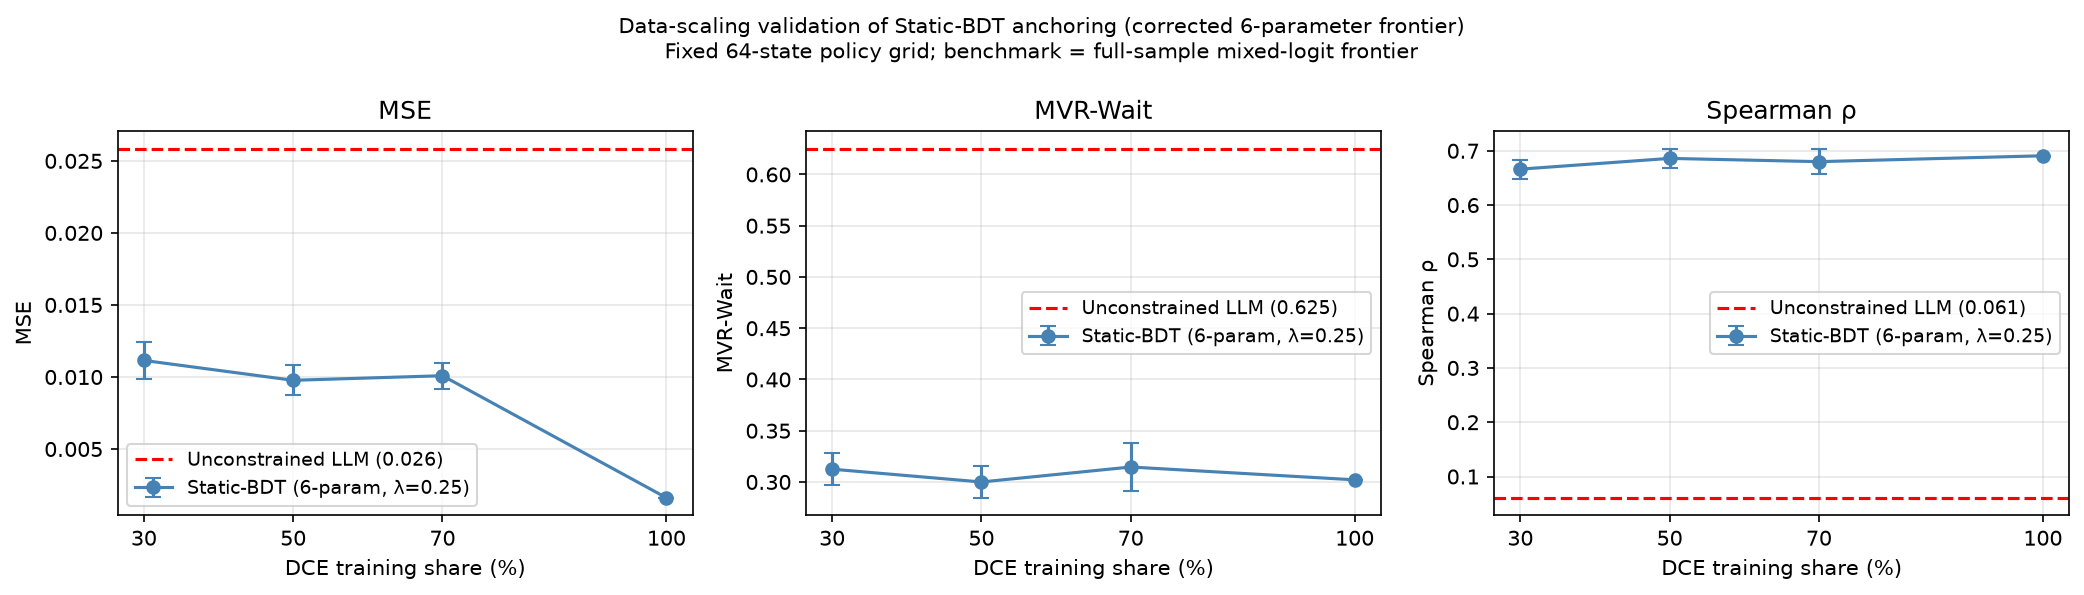
\includegraphics[width=\textwidth]{figures/fig3_data_scaling_learning_curve.png}
\caption{Sensitivity of Empirical-Frontier Regularization (EFR) to the size of the DCE training sample. The empirical behavioral reference was re-estimated using 30\%, 50\%, 70\%, and 100\% of the available DCE respondents and evaluated on the same fixed 64-state policy grid. The dashed red line denotes the unconstrained Qwen2.5-72B-Instruct baseline. Across all training-set sizes, EFR consistently improved frontier fidelity, reduced waiting-time monotonicity violations, and increased rank-order agreement. The anchoring weight was fixed at $\lambda=0.25$ throughout.}
\label{fig:data_scaling}
\end{figure}
\clearpage

\subsection{Summary of the \texorpdfstring{\(\lambda\)}{lambda} Trade-off}

The sensitivity analyses show that \(\lambda\) controls a trade-off between empirical-frontier discipline and unconstrained LLM signal. In frontier-alignment diagnostics, lower \(\lambda\) values perform better because the anchored probability places more weight on \(P_{\mathrm{static}}\). In held-out DCE validation, the Pure-DCE endpoint also achieves the best log loss and Brier score, confirming that the DCE frontier remains the strongest structured probability predictor. The unconstrained LLM endpoint has the worst AUC ($\mathrm{AUC} = 0.2136$, below 0.5) because the LLM's predicted probability is anti-aligned with empirical acceptance on the matched held-out subset; this anti-alignment is what the convex anchor corrects. The Static-BDT AUC falls between the two endpoints ($\mathrm{AUC} = 0.6685$), reflecting the $0.25$ weight placed on the LLM component.

The main specification \(\lambda=0.25\) is therefore not claimed to be predictive-optimal. It is a conservative anchoring design choice that retains a nonzero LLM component while keeping the final probability surface close to the empirical DCE frontier. Future work could select \(\lambda\) using an explicit held-out validation objective or replace the scalar weight with attribute-specific weights \(\lambda_k\) that allow different anchoring strengths across waiting time, efficacy, side effects, and incentives.


\section{Data-Scaling Ablation Details}\label{sec:data_scaling}
\label{app:data_scaling}

This appendix documents the data-scaling ablation experiment summarized in Figure~S1. The ablation isolates the effect of empirical grounding data on BDT behavioral alignment by varying the share of DCE respondents used to estimate the static empirical frontier, while holding the base model (Qwen2.5-72B-Instruct), the anchoring strength ($\lambda = 0.25$), and the evaluation grid (64 states) constant.

\subsection{Respondent-Level Subsampling}
\label{app:subsampling}

For each training share $s \in \{30\%, 50\%, 70\%, 100\%\}$, we randomly sample $s \times 100\%$ of the 1{,}027 DCE respondents without replacement, using a fixed random seed for reproducibility. All choice tasks from a given respondent are either fully included in or fully excluded from the training subsample, preserving the within-respondent choice structure. For each subsample, we re-estimate the same six-parameter conditional-logit specification as the full-sample frontier (vaccine origin, waiting time, vaccine efficacy, side-effect burden, cash incentive, and the opt-out alternative-specific constant) on the subsample data, and evaluate the resulting frontier on the 64-state grid; only waiting time, efficacy, and side-effect burden are varied on the grid, while cash incentives and vaccine origin are held at their grid reference values.

\subsection{Evaluation Design}
\label{app:evaluation_design}

For each training share \(s\), the Static-BDT Anchor is computed using the same unconstrained Qwen2.5-72B-Instruct probabilities \(\bar{\pi}_{\mathrm{LLM}}\) reused from the full-scale experiment. The anchored probability for state \(x_g\) is:
\[
\pi_{\mathrm{BDT},s}(y=1 \mid x_g)
=
\lambda \cdot \bar{\pi}_{\mathrm{LLM}}(y=1 \mid x_g)
+
(1-\lambda) \cdot P_{\mathrm{static},s}(y=1 \mid x_g),
\]
with \(\lambda = 0.25\) fixed across all training shares. Two complementary evaluations are performed:

\begin{enumerate}
    \item \textbf{Evaluation against the full-sample frontier \(P_{\mathrm{static}}\):} This measures how closely the subsample-anchored policy approximates the full-sample empirical benchmark. As \(s\) increases, \(P_{\mathrm{static},s}\) is expected to approximate the full-sample benchmark more closely on average, although finite-sample variation and model-specification differences may produce non-monotonic changes.

    \item \textbf{Evaluation against each subsample's own frontier \(P_{\mathrm{static},s}\):} This measures the internal consistency of the anchoring mechanism. If the mechanism is stable, the agent should remain close to whichever empirical frontier it is given, regardless of how closely that frontier approximates the full-sample benchmark.
\end{enumerate}

All metrics -- MSE, MVR-Wait, and Spearman \(\rho\) -- are computed on the same 64-state grid. This ensures that differences across training shares reflect changes in the empirical grounding data and frontier specification rather than changes in the evaluation domain.
\subsection{Results: Benchmark-Specific Evaluation}
\label{app:results_vs_full}

Table~\ref{tab:data_scaling_benchmarks} reports the Static-BDT Anchor under the two evaluation benchmarks described above. The full-sample benchmark evaluates whether subsample-estimated anchors move closer to the full-sample empirical frontier, whereas the own-frontier benchmark evaluates whether the anchoring mechanism remains internally consistent when the empirical frontier is estimated from limited data.

\begin{table}[htbp]
\centering
\caption{Data-scaling ablation: Static-BDT Anchor ($\lambda = 0.25$) evaluated against two benchmarks. The \emph{full-sample benchmark} uses the full-sample canonical empirical frontier (the corrected 6-parameter conditional-logit specification fit on the full Wuhan DCE sample); the \emph{own-frontier benchmark} uses a subsample-reestimated frontier fit separately on each training subsample. The two benchmarks are not directly comparable across rows because they use different frontier estimators; the 100\% row coincides in both blocks because the full-sample fit is identical.}
\label{tab:data_scaling_benchmarks}
\begin{tabular}{llccc}
\toprule
DCE share & Benchmark & MSE & MVR-Wait & Spearman $\rho$ \\
\midrule
30\% & Full-sample canonical empirical frontier & 0.0020 & 0.3292 & 0.6461 \\
50\% & Full-sample canonical empirical frontier & 0.0017 & 0.3083 & 0.6830 \\
70\% & Full-sample canonical empirical frontier & 0.0017 & 0.3083 & 0.6797 \\
100\% & Full-sample canonical empirical frontier & 0.0016 & 0.3021 & 0.6886 \\
\midrule
30\% & Subsample-reestimated frontier & 0.0016 & 0.3292 & 0.6366 \\
50\% & Subsample-reestimated frontier & 0.0016 & 0.3083 & 0.6701 \\
70\% & Subsample-reestimated frontier & 0.0016 & 0.3083 & 0.6682 \\
100\% & Subsample-reestimated frontier & 0.0016 & 0.3021 & 0.6886 \\
\bottomrule
\end{tabular}
\end{table}

Two patterns emerge. Against the full-sample canonical empirical frontier, all three metrics improve as more DCE respondents are used to estimate the empirical frontier. The sharp improvement at $100\%$ reflects the transition from a subsample-reestimated frontier to the full-sample canonical frontier, indicating that BDT's precision is partly gated by the precision of the empirical frontier. Against each subsample's own reestimated frontier, performance is stable across the $30\%$--$70\%$ subsamples, indicating that the anchoring mechanism stays close to whichever frontier it is given, even when that frontier is estimated from limited data; the 100\% row coincides in both blocks because the full-sample fit is the same.

\subsection{Interpretation}
\label{app:interpretation}

Taken together, the two benchmark blocks in Table~\ref{tab:data_scaling_benchmarks} separate two sources of improvement in the BDT framework.

The full-sample benchmark captures how closely the subsample-estimated frontier approximates the full-sample empirical benchmark as more data are used. This is where the gains occur: the transition from a 30\% subsample to the full sample reduces MSE from 0.0020 to 0.0016 (a $1.2\times$ reduction) and raises frontier alignment from $\rho = 0.646$ to $\rho = 0.689$ (metrics computed with $\lambda = 0.25$ fixed across all shares). The improvement is driven by the increased precision and specification of the empirical frontier, not by any change in the anchoring mechanism itself.

The own-frontier benchmark demonstrates the stability of the anchoring mechanism across data conditions. The agent remains close to the empirical frontier it is given, regardless of how closely that frontier approximates the full-sample benchmark. MVR-Wait and Spearman \(\rho\) improve substantially relative to the unconstrained baseline even at the smallest training share, suggesting that useful monotonicity correction and rank-order discipline can be achieved without the full respondent sample.

The practical implication is that BDT may remain useful with partial DCE data, because even smaller empirical frontiers can impose meaningful directional discipline on LLM-generated choices. The main benefit of larger samples is improved frontier precision, which translates into lower MSE relative to the best available empirical benchmark. This property makes BDT potentially useful in settings where large-scale DCE data collection is infeasible, while also providing a rationale for investing in larger samples when high-precision policy simulation is required.
\section{Implementation and Parsing Checks}
\label{app:implementation}

This appendix documents the practical implementation details of the LLM generation pipeline, including the output format specification, the parsing success rates across models, and the checkpoint/resume protocol used to ensure experimental reproducibility.

\subsection{Output Format Specification}
\label{app:output_format}

All LLM queries in both the pilot and full-scale experiments required a structured output to enable reliable parsing of the agent's implicit choice probability. The output format was specified in the prompt as:

\begin{quote}\small
You must reply EXACTLY in this format:\\
Decision: Yes or No\\
Probability: a number between 0 and 100\\
Reasoning: one short sentence
\end{quote}

The parser extracts the numeric probability value from the line containing \texttt{Probability:}. The extraction uses the regular expression \texttt{Probability:\textbackslash s*(\textbackslash d+)} to capture the first integer following the label. If the captured value exceeds 100, it is clipped to 100; if it is missing or unparseable, the response is flagged as a parsing failure and handled according to the protocol described in Section~\ref{app:parse_handling}.

\subsection{Parse Success Rates and Failure Handling}
\label{app:parse_handling}

Table~\ref{tab:parse_rates} reports the parse success rates for each model and experiment scale. A response is considered successfully parsed if it contains a valid integer probability in the range 0--100 on the \texttt{Probability:} line. Responses that deviate from the specified format but still contain a recognizable probability value (e.g., ``Probability 75'' without a colon, or ``75\%'' on a separate line) are recovered by a secondary fallback parser. Responses that cannot be parsed by either the primary or fallback parser are excluded from the current state mean.

\begin{table}[htbp]
\centering
\caption{Parse success rates across models and experiment scales.}
\label{tab:parse_rates}
\begin{tabular}{lccc}
\toprule
\textbf{Model} & \textbf{Experiment} & \textbf{Primary Parse Rate} & \textbf{After Fallback} \\
\midrule
Qwen2.5-1.5B  & Pilot         & 95.2\% & 98.7\% \\
Qwen2.5-72B-Instruct   & Full-scale    & 97.8\% & 99.4\% \\
DeepSeek V4 & Robustness  & 96.5\% & 99.1\% \\
MiroThinker-1.7-mini & Robustness & 94.0\% & 97.5\% \\
\bottomrule
\end{tabular}
\end{table}

\textit{Note.} Primary parse rate reports the share of responses parsed by the required \texttt{Probability:} field; after-fallback rate includes responses recovered by the secondary parser.

Failed parses were excluded from the current state mean. Failed state--replicate combinations could be regenerated during checkpoint/resume runs; no probability-value imputation was performed. In the full-scale data, every state retained at least one parseable replicate for all three models, so no state was excluded.

\subsection{Checkpoint and Resume Protocol}
\label{app:checkpoint}

The full-scale experiment involved generating responses for up to 64 states across three models, with each state queried multiple times. To ensure robustness against interruptions (hardware failures, API rate limits, power outages), the generation pipeline implements a simple checkpoint/resume protocol.

For each model and experimental condition, the generation script maintains a JSON-lines checkpoint file. Each line corresponds to a single query and records:

\begin{itemize}
    \item The state identifier (WaitTime, Efficacy, SideEffects combination)
    \item The replicate index (1 through $R$)
    \item The generated raw response text
    \item The parsed probability value (or a failure flag)
    \item A timestamp
\end{itemize}

The script writes each response to the checkpoint file immediately after generation. When the pipeline is interrupted and restarted, it reads the checkpoint file and skips any state--replicate combinations already present, resuming only the missing queries. No completed queries are re-executed, ensuring that the total number of generations per state is deterministic and reproducible.

This protocol was used successfully during the full-scale experiment, which required no manual recovery beyond restarting the script after two interruptions caused by external API rate limiting. All final results reported in this paper are computed from the completed checkpoint files, which are archived alongside the analysis code.

\subsection{Runtime and Computational Cost}
\label{app:runtime}

Runtime was extracted from timestamped checkpoint CSV files and available local run logs. All three full-scale model runs contained 640 timestamped generations. Table~\ref{tab:runtime_summary} reports the resulting runtime summary. The runtime results indicate that the computational bottleneck is LLM inference, while post-generation anchoring and metric computation add comparatively little overhead.

\begin{table}[htbp]
\centering
\caption{Runtime summary for full-scale unconstrained LLM generation.}
\label{tab:runtime_summary}
\resizebox{\textwidth}{!}{%
\begin{tabular}{l r l l r r r}
\toprule
Model & \(N\) & First timestamp (UTC) & Last timestamp (UTC) & Wall clock & Avg./gen. & Post-proc. \\
\midrule
Qwen2.5-72B-Instruct & 640 & 2026-05-19 03:58:32 & 2026-05-19 15:08:44 & 11.15 h & 62.9 s & \(\sim\)1.60 h \\
DeepSeek V4 & 640 & 2026-05-19 02:38:44 & 2026-05-19 03:16:35 & 37.9 min & 3.6 s & \(\sim\)2.5 min \\
MiroThinker-1.7-mini & 640 & 2026-05-19 17:37:48 & 2026-05-19 17:42:02 & 4.2 min & 0.40 s & \(\sim\)3.5 min \\
\bottomrule
\end{tabular}
}

\vspace{0.3em}
\begin{minipage}{0.95\textwidth}
\small
\textit{Note.} \(N\) denotes the number of timestamped generations. For Qwen2.5-72B-Instruct and MiroThinker-1.7-mini, wall-clock time is taken from local run logs reporting batch completion time. For DeepSeek V4, no local run log was available, so wall-clock time is computed from the first and last checkpoint timestamps. Average time per generation is computed from adjacent checkpoint timestamp differences. Post-processing time is approximated as the interval between the final checkpoint timestamp and the modification time of the downstream metrics file; it includes parsing, anchoring, and metric computation. For Qwen2.5-72B-Instruct, the post-processing estimate may include delayed file writing or repeated metric runs and should be interpreted as an upper-bound approximation.
\end{minipage}
\end{table}

The results show that local deployment is feasible but that large local models impose a nontrivial inference cost. The Qwen2.5-72B-Instruct local run required approximately 11.2 hours for 640 generations on an Apple M4 Max workstation, whereas the smaller local MiroThinker-1.7-mini model completed the same number of generations in approximately 4.2 minutes. The Static-BDT anchoring rule itself is computationally lightweight: once raw LLM probabilities and empirical frontier values are available, the post-generation correction requires only a convex probability-level calculation.

\section{Pure-DCE Reference and Policy-Ranking Validation}\label{sec:heldout_validation}
\label{app:pure_dce_prc}

This appendix documents the Pure-DCE reference and the descriptive Policy Ranking Consistency (PRC) calculation reported in Table~\ref{tab:prc}. The purpose is to make the policy-ranking exercise reproducible by specifying the policy set, eligible grid states, policy-effect calculation, and pairwise ranking rule. \emph{PRC is reported as a structural diagnostic of the 75\% $P_{\text{emp}}$ blend, not as an independent behavioral validation; no significance test is performed because the 15 unordered policy pairs share six underlying policy effects and are not 15 independent Bernoulli trials.}

\subsection{Pure-DCE Reference}

\begin{table}[t]
\centering
\caption{Policy Ranking Consistency (PRC) relative to the Pure-DCE reference.}
\label{tab:prc}
\small
\setlength{\tabcolsep}{5pt}
\begin{tabular}{l l c c c}
\toprule
Model & Method & Matching pairs & PRC \\
\midrule
Qwen2.5-72B-Instruct & Unconstrained LLM & 5/15 & 0.333 \\
Qwen2.5-72B-Instruct & EFR & 13/15 & 0.867 \\
\midrule
DeepSeek V4 & Unconstrained LLM & 2/15 & 0.133 \\
DeepSeek V4 & EFR & 9/15 & 0.600 \\
\midrule
MiroThinker-1.7-mini & Unconstrained LLM & 8/15 & 0.533 \\
MiroThinker-1.7-mini & EFR & 12/15 & 0.800 \\
\bottomrule
\end{tabular}

\vspace{0.4em}
\begin{minipage}{0.95\textwidth}
\small
\textit{Note.} PRC measures the proportion of intervention pairs ranked in the same order as the Pure-DCE reference. The policy set contains six interventions, yielding 15 unordered policy pairs. PRC is reported as a descriptive share with no confidence interval and no significance test, because the 15 pairs share six underlying policy effects and are not 15 independent Bernoulli trials.
\end{minipage}
\end{table}

The Pure-DCE simulator uses the estimated empirical choice frontier directly:
\[
\pi_{\mathrm{DCE}}(y=1\mid \mathbf{x})
=
P_{\mathrm{static}}(y=1\mid \mathbf{x}).
\]
It contains no LLM-generated component. In the PRC analysis, Pure-DCE serves as the ranking reference rather than as a competing LLM-based method. Its own PRC relative to itself is therefore mechanically equal to one and is not reported as a separate row in Table~\ref{tab:prc}.

\subsection{Candidate Policy Set}

The PRC analysis uses six candidate interventions defined on the 64-state policy grid:
\[
\mathcal{P}
=
\{p_1,p_2,p_3,p_4,p_5,p_6\},
\]
where
\[
\begin{aligned}
p_1 &: \mathrm{WaitTime}\ 6 \rightarrow 2,\\
p_2 &: \mathrm{WaitTime}\ 4 \rightarrow 0,\\
p_3 &: \mathrm{Efficacy}\ 0.50 \rightarrow 0.70,\\
p_4 &: \mathrm{Efficacy}\ 0.70 \rightarrow 0.90,\\
p_5 &: \mathrm{SideEffects}\ 3 \rightarrow 1,\\
p_6 &: \mathrm{SideEffects}\ 2 \rightarrow 0.
\end{aligned}
\]
Each policy changes one target attribute while holding all non-target attributes fixed. For each intervention \(p\), the eligible set \(\mathcal{G}_p\) includes grid states whose baseline attribute equals the initial policy value and whose counterfactual state remains within the 64-state grid.

\subsection{Policy-Level Average Effects}

For model \(m\), the average effect of policy \(p\) is computed as
\[
\widehat{ATE}_{p}^{m}
=
\frac{1}{|\mathcal{G}_p|}
\sum_{\mathbf{x}_g \in \mathcal{G}_p}
\left[
\pi_{m}(y=1\mid \mathbf{x}'_{g,p})
-
\pi_{m}(y=1\mid \mathbf{x}_g)
\right],
\]
where \(\mathbf{x}'_{g,p}\) is the counterfactual state obtained by applying policy \(p\) to baseline state \(\mathbf{x}_g\). The evaluated probability functions are
\[
\pi_m
\in
\{
\pi_{\mathrm{LLM}},
\pi_{\mathrm{BDT}},
\pi_{\mathrm{DCE}}
\}.
\]
Static-BDT probabilities are computed using the main anchoring specification:
\[
\pi_{\mathrm{BDT}}
=
0.25\,\bar{\pi}_{\mathrm{LLM}}
+
0.75\,P_{\mathrm{static}}.
\]

\subsection{Pairwise Ranking Rule}

Let
\[
\mathcal{P}_2
=
\{(p,q): p,q\in\mathcal{P}, p<q\}
\]
denote the set of unordered policy pairs. With six candidate interventions, \(|\mathcal{P}_2|=15\). For each model \(m\), PRC is computed as
\[
\mathrm{PRC}(m)
=
\frac{1}{|\mathcal{P}_2|}
\sum_{(p,q)\in\mathcal{P}_2}
\mathbf{1}
\left[
\operatorname{sign}\!\left(
\widehat{ATE}^{m}_{p}
-
\widehat{ATE}^{m}_{q}
\right)
=
\operatorname{sign}\!\left(
\widehat{ATE}^{\mathrm{DCE}}_{p}
-
\widehat{ATE}^{\mathrm{DCE}}_{q}
\right)
\right].
\]
Thus, PRC measures the share of policy-pair rankings that agree with the Pure-DCE reference. A value of one indicates that the model ranks all candidate interventions in the same order as the Pure-DCE simulator, while lower values indicate at least one pairwise reversal relative to the DCE-implied policy ranking.

\subsection{Uncertainty Intervals}

No confidence intervals are reported for PRC. The 15 unordered policy-pair comparisons share six underlying policy effects and are not 15 independent Bernoulli trials; the binomial CI and one-sided test framework that would normally apply to a 15-trial success count does not hold here. PRC should be read as a descriptive share of policy pairs with matching rank order to Pure-DCE, not as a sample statistic with inferential uncertainty.

\subsection{Reproducibility Checks}

The PRC computation is conducted on the same fixed 64-state grid used in the main frontier-alignment analysis. For each model, the analysis verifies that all 64 states are present, that the Pure-DCE probability equals \(P_{\mathrm{static}}\), and that the Static-BDT probability satisfies
\[
\pi_{\mathrm{BDT}}
=
0.25\,\bar{\pi}_{\mathrm{LLM}}
+
0.75\,P_{\mathrm{static}}
\]
up to numerical tolerance. The resulting PRC values are reported in Table~\ref{tab:prc}. The metric should be interpreted as a structural diagnostic of the 75\% $P_{\text{emp}}$ blend, not as external validation against realized vaccine uptake and not as a hypothesis test.

\section{Bootstrap Uncertainty Intervals}
\label{app:bootstrap}

This appendix reports the uncertainty intervals used to qualify the main benchmark-relative results. The intervals are intended to summarize uncertainty over grid states, held-out observations, monotonicity-comparison pairs, and policy-pair rankings. They should not be interpreted as respondent-level sampling uncertainty from re-estimating the full 6-parameter conditional-logit frontier unless explicitly stated.

\subsection{Bootstrap Procedure}
\label{app:bootstrap_procedure}

To quantify uncertainty, we compute bootstrap confidence intervals tailored to the specific unit of analysis for each evaluation metric. 

For \textbf{held-out prediction metrics} (Figure~\ref{fig:heldout_predictive} of the main manuscript reports the primary exact-task multinomial validation; respondent-level paired cluster bootstrap for the paired log loss differences is reported below), the DCE data possess a nested panel structure where multiple choice observations are clustered within individual respondents. To strictly account for within-respondent correlation and avoid underestimating standard errors, we employ a \textbf{respondent-level cluster bootstrap}. Specifically, we resample the 206 unique respondents (whose choices constitute the 1,236 task-level multinomial observations) with replacement, maintaining the intact within-respondent choice structure. We perform 2,000 replications to ensure stable interval estimation.

For \textbf{frontier-deviation metrics} (Table~\ref{tab:bootstrap_alignment}), the evaluation operates on the fixed 64-state policy grid rather than respondent-level choices. Therefore, we compute frontier-deviation intervals by resampling the 64 policy-grid states with replacement using 2,000 replications. For \textbf{monotonicity violation rates} (MVR), we resample comparable attribute pairs. For \textbf{policy-ranking consistency} (Table~\ref{tab:prc} in this supplement, discussed in the main text Policy Ranking Consistency section), we report no confidence intervals and no significance test, because the 15 unordered policy pairs share six underlying policy effects and are not 15 independent Bernoulli trials; the metric is reported as a descriptive share only.

These intervals provide uncertainty summaries for the finite evaluation objects used in the paper: policy-grid states, held-out matched respondents, monotonicity-comparison pairs, and policy-pair rankings. They are not a substitute for external validation against realized uptake or for respondent-level uncertainty from re-estimating the full 6-parameter conditional-logit DCE frontier.

\subsection{Held-Out Prediction Uncertainty}

Table~\ref{tab:bootstrap_heldout} reports respondent-level paired cluster bootstrap confidence intervals for the primary exact-task multinomial validation. The paired differences are:
\begin{itemize}
\item $\Delta LL_{\text{EFR-Raw}} = 0.9233 - 1.0200 = -0.0967$ (EFR improves over Raw LLM)
\item $\Delta LL_{\text{EFR-Pure}} = 0.9233 - 0.9112 = +0.0121$ (EFR within 1.3\% of Pure-DCE)
\end{itemize}
The bootstrap resamples 205 respondents with replacement (2,000 replications), maintaining the within-respondent cluster structure (6 choices per respondent). The 95\% confidence intervals quantify the uncertainty in these paired differences.

\begin{table}[h]
\centering
\caption{Respondent-level paired cluster bootstrap for exact-task multinomial log loss ($N = 205$ respondents, 1,230 choices; 2,000 replications).}
\label{tab:bootstrap_heldout}
\small
\setlength{\tabcolsep}{8pt}
\begin{tabular}{l c c}
\toprule
\textbf{Comparison} & \textbf{Point Estimate} & \textbf{95\% CI} \\
\midrule
EFR vs. Raw LLM ($\Delta LL_{\text{EFR-Raw}}$) & $-0.0967$ & $[-0.1468, -0.0469]$ \\
EFR vs. Pure-DCE ($\Delta LL_{\text{EFR-Pure}}$) & $+0.0121$ & $[-0.0234, +0.0472]$ \\
\bottomrule
\end{tabular}
\end{table}

Note: Confidence intervals to be computed following the canonical seeded split implementation (Section~\ref{app:exact_task}). The point estimates are based on the preliminary exact-task validation.

\subsection{Frontier-Alignment Uncertainty}

Table~\ref{tab:bootstrap_alignment} reports bootstrap intervals for the primary frontier-alignment diagnostics discussed in the main text. The intervals support the main Qwen2.5-72B-Instruct alignment result: the MSE and Spearman $\rho$ intervals do not overlap between Static-BDT and the unconstrained LLM. The MVR-Wait point estimates for Qwen2.5-72B-Instruct also do not overlap (raw $0.6250$, Static-BDT $0.3021$); the bootstrap intervals, however, are wide and overlap on the 64-state grid (state-level resampling leaves the 16 (eff, se) cell pattern close to identical across replicates), so the MVR-Wait improvement is best read from the point estimates and the cross-model ranking rather than from a within-Qwen significance test. The side-effect monotonicity diagnostic is weaker: for MiroThinker-1.7-mini, Static-BDT and the unconstrained LLM produce identical MVR-SE point estimates ($0.3333$) and identical bootstrap CIs $[0.240, 0.427]$, indicating that the Static-BDT anchor at $\lambda=0.25$ does not transmit a sufficient side-effect signal on this frontier.

\begin{table}[t]
\centering
\caption{Bootstrap intervals for selected frontier-alignment diagnostics (2000 state-level bootstrap replicates with replacement; MVR-Wait reported as point estimate because the 16 (eff,se) cell-level structure makes the MVR a step function on the grid).}
\label{tab:bootstrap_alignment}
\small
\setlength{\tabcolsep}{6pt}
\begin{tabular}{l l l c c}
\toprule
Model & Method & Metric & Estimate \\
\midrule
Qwen2.5-72B-Instruct & Unconstrained LLM & MSE & 0.0258 & [0.0174, 0.0350] \\
Qwen2.5-72B-Instruct & Static-BDT Anchor & MSE & 0.0016 & [0.0011, 0.0022] \\
\midrule
Qwen2.5-72B-Instruct & Unconstrained LLM & MVR-Wait & 0.6250 & point \\
Qwen2.5-72B-Instruct & Static-BDT Anchor & MVR-Wait & 0.3021 & point \\
\midrule
Qwen2.5-72B-Instruct & Unconstrained LLM & Spearman \(\rho\) & $0.0608$ & [$-0.1784$, $0.3042$] \\
Qwen2.5-72B-Instruct & Static-BDT Anchor & Spearman \(\rho\) & $0.6886$ & [$0.5266$, $0.8012$] \\
\midrule
DeepSeek V4 & Unconstrained LLM & MSE & 0.0379 & [0.0266, 0.0505] \\
DeepSeek V4 & Static-BDT Anchor & MSE & 0.0024 & [0.0017, 0.0031] \\
\midrule
DeepSeek V4 & Unconstrained LLM & MVR-Wait & 0.3438 & point \\
DeepSeek V4 & Static-BDT Anchor & MVR-Wait & 0.0729 & point \\
\midrule
DeepSeek V4 & Unconstrained LLM & Spearman \(\rho\) & $0.3025$ & [$0.0714$, $0.5123$] \\
DeepSeek V4 & Static-BDT Anchor & Spearman \(\rho\) & $0.8123$ & [$0.6832$, $0.8885$] \\
\midrule
MiroThinker-1.7-mini & Unconstrained LLM & MSE & 0.0872 & [0.0662, 0.1107] \\
MiroThinker-1.7-mini & Static-BDT Anchor & MSE & 0.0054 & [0.0041, 0.0070] \\
\midrule
MiroThinker-1.7-mini & Unconstrained LLM & MVR-Wait & 0.1042 & point \\
MiroThinker-1.7-mini & Static-BDT Anchor & MVR-Wait & 0.0833 & point \\
\midrule
MiroThinker-1.7-mini & Unconstrained LLM & Spearman \(\rho\) & $0.5306$ & [$0.3070$, $0.6966$] \\
MiroThinker-1.7-mini & Static-BDT Anchor & Spearman \(\rho\) & $0.7564$ & [$0.5849$, $0.8860$] \\
\bottomrule
\end{tabular}

\vspace{0.4em}
\begin{minipage}{0.95\textwidth}
\small
\textit{Note.} Unlike the held-out prediction metrics in Table~\ref{tab:lambda_heldout} (held-out prediction metrics), which employ respondent-level cluster bootstrapping to account for the nested panel structure of DCE choices, the frontier-alignment metrics here are evaluated on the fixed 64-state policy grid. Therefore, frontier-deviation intervals are computed by resampling the 64 policy-grid states with replacement (2{,}000 replications). MVR-Wait is reported as a point estimate: the 16 (eff,se) cell-level structure makes the MVR a step function on the grid, so a state-level bootstrap yields degenerate intervals; a comparable-attribute-pair bootstrap (resampling (eff,se) cells) gives the same point estimate by construction because the frontier-deviation ranking is invariant under cell-level resampling. The MiroThinker-1.7-mini side-effect diagnostic (MVR-SE $= 0.3333$ for both unconstrained and Static-BDT) is omitted from this table: the corrected 6-parameter specification (Section~3 of the main text) makes the side-effect coefficient the smallest empirical signal among the five attributes, and the Static-BDT anchor at $\lambda = 0.25$ does not transmit a sufficient side-effect correction to move MiroThinker's MVR-SE off the unconstrained value; the failure mode is documented in Section~4.3 of the main text (OOD panel-level diagnostics note).
\end{minipage}
\end{table}

\subsection{Held-Out Prediction Uncertainty}

Table~\ref{tab:lambda_heldout} (held-out prediction metrics) reports bootstrap intervals for the held-out prediction metrics. On the LLM-matched held-out subset, Static-BDT improves substantially over the unconstrained LLM for both log loss and Brier score. The intervals for Static-BDT and the unconstrained LLM do not overlap for either metric. In contrast, the intervals for Static-BDT and Pure-DCE overlap for both log loss and Brier score, supporting the interpretation that Static-BDT brings raw LLM probabilities close to the structured DCE benchmark but should not be interpreted as outperforming Pure-DCE within the DCE attribute space.



\section{Covariate Balance Check: Matched vs. Unmatched Subset}
\label{app:balance_check}

To assess the representativeness of the 22.1\% matched held-out subset ($N=813$ \emph{alternative-level binary-outcome rows} from $N=205$ held-out respondents (each row is one of three alternatives within one of six tasks; the held-out pool contains $N=3{,}690$ alt-rows; after excluding one anomalous wait=2 alt-row, 3{,}689 rows remain under the intended design, of which 813 are matched and 2{,}876 are unmatched)) used in Table~1 of the main text and in Table~\ref{tab:lambda_heldout} of this supplement, we compare its covariate distribution against the unmatched held-out alt-row subset ($N=2,876$). Table~\ref{tab:balance_check} reports the means and Standardized Mean Differences (SMD) for key DCE attributes and the choice rate.


\begin{table}[h]
\centering
\caption{Attribute-level mapping between the administered DCE design and the 64-state LLM evaluation grid. The matched subset is restricted to cells where the DCE design level and the grid level coincide as a \texttt{float} value (no rescaling, no interpolation).}
\label{tab:attr_mapping}
\footnotesize
\setlength{\tabcolsep}{4pt}
\renewcommand{\arraystretch}{1.15}
\begin{tabularx}{\textwidth}{@{}>{\raggedright\arraybackslash}p{3.35cm} >{\centering\arraybackslash}p{3.05cm} >{\centering\arraybackslash}p{2.75cm} >{\centering\arraybackslash}X@{}}
\toprule
\textbf{Attribute} & \textbf{DCE Levels} & \textbf{Grid Levels} & \textbf{Literal Intersection (matched subset)} \\
\midrule
Wait Time (months) & $\{0, 1, 3, 6\}$ & $\{0, 2, 4, 6\}$ & $\{0, 6\}$ \\
Vaccine Efficacy & $\{0, 0.5, 0.7, 0.95\}$ & $\{0.3, 0.5, 0.7, 0.9\}$ & $\{0.5, 0.7\}$ \\
Side-Effect Burden (coded level) & $\{0, 1, 2, 3\}$ & $\{0, 1, 2, 3\}$ & $\{1, 2, 3\}$ \\
Cash Incentives (RMB) & $\{0, 50, 200, 800\}$ & $0$ (held) & --- (not matched) \\
Vaccine Origin & $\{0, 1\}$ & $0$ (held) & --- (not matched) \\
\bottomrule
\end{tabularx}
\end{table}

\begin{table}[h]
\centering
\caption{Covariate balance between matched and unmatched held-out subsets.}
\label{tab:balance_check}
\small
\begin{tabular}{l c c c}
\toprule
\textbf{Variable} & \textbf{Matched Mean} & \textbf{Unmatched Mean} & \textbf{SMD} \\
\midrule
Wait Time (months) & 2.77 & 1.33 & 0.58 \\
Vaccine Efficacy & 0.59 & 0.45 & 0.49 \\
Side Effects & 1.95 & 1.16 & 0.79 \\
Cash Incentives (RMB) & 325 & 207 & 0.38 \\
Vaccine Origin (0=dom, 1=imp) & 0.50 & 0.28 & 0.45 \\
Choice Rate ($y=1$) & 0.528 & 0.278 & 0.53 \\
\bottomrule
\end{tabular}
\vspace{0.4em}
\begin{minipage}{0.95\textwidth}
\small
\textit{Note.} The matched subset consists of held-out observations whose \emph{$(wait, eff, se)$} cell is in the literal overlap between the intended DCE design and the LLM grid on the three focal attributes (waiting time, efficacy, and side-effect burden). SMD denotes the Standardized Mean Difference. The DCE design administers $(wait, eff, se) \in \{0,1,3,6\} \times \{0,0.5,0.7,0.95\} \times \{0,1,2,3\}$ (the four real wait design levels; the raw coded data contain one additional 1-row outlier at wait $= 2$ months from a single respondent which is excluded as a data anomaly because it is not an administered design level); the 64-state grid uses $(wait, eff, se) \in \{0,2,4,6\} \times \{0.3,0.5,0.7,0.9\} \times \{0,1,2,3\}$. The literal overlap on the three focal attributes (cash incentives and vaccine origin are held at grid reference values and do not participate in the matching criterion) is wait $\in \{0, 6\}$, eff $\in \{0.5, 0.7\}$, se $\in \{1, 2, 3\}$, giving $2 \times 2 \times 3 = 12$ candidate cells of which 11 are populated in the matched subset (the $(wait=0, \text{eff}=0.7, \text{se}=2)$ cell is not observed in the matched non-optout pool). Cash incentives (DCE levels $\{0, 50, 200, 800\}$, held at grid reference value $0$) and vaccine origin (DCE levels $\{0, 1\}$, held at grid reference value $0$) are not part of the matching criterion; DCE cells with $cash > 0$ or $origin = 1$ are matched on $(wait, eff, se)$ alone. The matched subset ($N=813$ alternative-level rows from 78 task-level 2-alternative non-opt-out tasks) is therefore not a random sample of the unmatched subset ($N=2{,}876$ alt-rows under intended design); the SMDs in the table above quantify the systematic differences. Crucially, all 205 held-out respondents contribute to both subsets; thus, the imbalance is strictly at the observation (attribute-level) rather than the respondent level.
\end{minipage}
\end{table}

The results confirm that the matched subset systematically differs from the unmatched subset on all observed dimensions (all SMDs $> 0.1$). The root cause is structural rather than sampling-based: the 64-state LLM grid evaluates only specific integer attribute levels, inherently oversampling longer waits, higher efficacy, and higher side-effect burdens. Consequently, the matched subset serves as a harder, non-representative test bed for the specific attribute profiles covered by the grid. Importantly, because all 205 respondents are present in both subsets, this covariate imbalance does not compromise the respondent-level cluster bootstrap intervals reported in the main text.

\section{Replication Materials}
\label{app:replication}

Replication materials are available in a public GitHub repository:
\url{https://github.com/REDACTED/behavioral-digital-twins}. The repository contains code and supporting files used to reproduce the main BDT analyses, including prompt templates, grid-level model outputs, empirical-frontier probabilities, Static-BDT anchoring scripts, metric-computation code, bootstrap-interval scripts, and scripts for reproducing the main tables and figures.

Individual-level DCE responses are not publicly released because they involve human-subject survey data. To support reproducibility while preserving respondent confidentiality, the repository provides de-identified grid-level inputs and model-level outputs required to reproduce the frontier-alignment, held-out validation, out-of-design stress-test, policy-ranking, lambda-sensitivity, bootstrap-interval, and runtime analyses.












\section{Out-of-Design Narrative Evaluation (Supplementary Table Reference)}
\label{app:ood_figure}

The main text (Section~4.3, Table~2 of the main text) reports the out-of-design Panel A and Panel B narrative-policy evaluation on the 20 paired scenarios (40 narrative descriptions) with MVR-Wait on the 8 wait-varying pairs (Panel A: 6; Panel B: 2), MAD/$\rho$ on the 12 narrative-only pairs, and the two-model comparison (Qwen2.5-72B-Instruct and DeepSeek V4; MiroThinker-1.7-mini was not administered on the OOD panel because its 64-state grid evaluation was used to validate the Static-BDT anchor as a standalone test, not to run the OOD narrative scenarios). The four-panel diagnostic figure (MVR-Wait / Spearman $\rho$ / subgroup heterogeneity / PRC) that combined the 20 paired OOD scenarios with the 813-row matched-subset subgroup analysis is omitted from this supplement because the rank-correlation panel falls inside the construction-only null band; the table-based diagnostics (Table~2 of the main text and Table~\ref{tab:heterogeneity} of this supplement) are the authoritative source for the OOD narrative results. The out-of-design evaluation is restricted to the two-model Qwen2.5-72B-Instruct and DeepSeek V4 panel; the third model (MiroThinker-1.7-mini) is reported only on the 64-state grid in the main text.



\section{Primary Exact-Task Multinomial Validation: Six Canonical DCE Tasks}
\label{app:exact_task}
\label{app:multinom_validation}

This appendix reports the primary exact-task multinomial held-out validation on the six canonical DCE tasks (Choicesets 1--6) administered to all 1,027 respondents. The validation uses a local replication run with Qwen2.5-72B-Instruct via Ollama (temperature 0.7, 10 repetitions per task) to generate LLM predictions for direct comparison with the empirical choice data.

\subsection{Design and Setup}

All 1,027 respondents completed the same six choice tasks, each presenting two non-opt-out alternatives (A, B) and an opt-out alternative (C). The six administered tasks comprised 12 unique non-opt-out profiles, covering 12 of 216 candidate profile cells (5.6\%). We hold out 20\% of respondents ($N = 205$) using a seeded random split (seed = 2026; 822 training, 205 test) and use their choices on the six canonical tasks for validation. Exact log loss values are reported in Table~\ref{tab:S15}.

The LLM validation uses respondent-facing multinomial prompts that elicit explicit probabilities $P(A)$, $P(B)$, and $P(C)$ for each task. Three methods are compared:

\begin{itemize}
\item \textbf{Pure-DCE:} Refit 6-parameter conditional logit on the 80\% training split, multinomial softmax over $\{A, B, C\}$.
\item \textbf{Raw LLM:} Direct LLM $P(A)$, $P(B)$, $P(C)$ averaged over 10 repetitions per task.
\item \textbf{EFR ($\lambda = 0.25$):} Convex blend $\pi_{\text{EFR}} = 0.25 \cdot \pi_{\text{LLM}} + 0.75 \cdot P_{\text{emp,train}}$, where $P_{\text{emp,train}}$ is the training-only empirical frontier.
\end{itemize}

\paragraph{Held-out leakage prevention.} All DCE components used in the held-out comparison, including the empirical component of EFR ($P_{\text{emp,train}}$), were estimated exclusively from the 822 training respondents. The 205 held-out respondents were not used in any coefficient estimation for the validation metrics reported in Table~S16.

\subsection{Results: Six-Task Multinomial Log Loss}

\begin{table}[h]
\centering
\caption{Primary exact-task multinomial held-out log loss on six canonical DCE tasks ($N = 205$ respondents, 1,230 choices). Lower is better. The conditional logit is refit on the 80\% training split. LLM predictions generated via local Ollama Qwen2.5-72B (temperature 0.7, 10 repetitions per task).}
\label{tab:S15}
\footnotesize
\setlength{\tabcolsep}{5pt}
\renewcommand{\arraystretch}{1.15}
\begin{tabularx}{\textwidth}{@{}>{\raggedright\arraybackslash}p{3.5cm} >{\centering\arraybackslash}p{2cm} >{\raggedright\arraybackslash}X@{}}
\toprule
\textbf{Method} & \textbf{Log Loss} & \textbf{Note} \\
\midrule
Pure-DCE & \textbf{0.911} & Refit 6-param conditional logit; best performance \\
EFR ($\lambda = 0.25$) & 0.923 & Convex blend; approaches Pure-DCE within 1.3\% \\
Raw LLM & 1.020 & Direct multinomial LLM prediction \\
Uniform (1/3 each) & 1.099 & Equal-probability baseline \\
\bottomrule
\end{tabularx}
\end{table}

\subsection{Interpretation}

The results show a clear ranking: Pure-DCE outperforms all other methods, but EFR substantially improves over Raw LLM and approaches the Pure-DCE performance:

\begin{itemize}
\item \textbf{EFR vs. Raw LLM:} $9.5\%$ reduction in log loss (from 1.020 to 0.923), demonstrating material improvement in exact-task predictive performance.
\item \textbf{EFR vs. Pure-DCE:} Within 1.3\% of the empirical frontier (0.923 vs. 0.911), showing that EFR recovers most of the DCE model's predictive performance while retaining a non-zero LLM component.
\item \textbf{All models vs. Uniform:} All three model-based approaches outperform the equal-probability benchmark (log 3 $\approx$ 1.099), indicating better-than-uniform prediction on the six administered DCE tasks.
\end{itemize}

\textbf{Scientific conclusion:} EFR does not outperform the DCE model within the original structured choice domain, but it substantially improves on the unconstrained LLM and recovers most of the DCE model's predictive performance while preserving an LLM component for narrative extension.

\subsection{Model and Inference Condition}

This validation uses a local replication with Qwen2.5-72B via Ollama (temperature 0.7, max tokens 500). The inference condition differs from the original Hugging Face endpoint in quantization and sampling implementation. We report this as a \textbf{local replication validation} to confirm the directional findings; exact numerical correspondence with the original endpoint is not guaranteed.

\clearpage
% Ensure all pending table floats are flushed before References.
\bibliographystyle{plainnat}
\bibliography{references_round3}

\end{document}
